\section{Overview over the pipeline}~\label{seg:ov_pip}

To overcome the two problems stated in the previous section, the following was done. Making hard decisions on merges and unmerges between superpixels is on the one hand bad, because one has to do a hard thresholding of a networks predictions which robs us from the information that lies within the uncertainty in the predictions. On the other hand contradictions can arise in the final segmentation. Both can be overcome by predicting pseudo probabilities for the edges between superpixels which can be transformed into costs and a multicut \ref{sec:multicut} of the superpixel graph can be computed. This leverages the uncertainty of the network predictions and overcomes contradictions in the segmentation. \\
The second issue that arises from the irregularity of the superpixel graph can be overcome by using a graph neural network that predicts edge weights between superpixels by performing graph convolutions \ref{sec:gcn}. However this generates the problem that there have to be regular representations for superpixels. Of course one solution would be to have two gcns, one for intra superpixel convolution and one for inter superpixel convolution. the former would take every pixel within a superpixel as a node with the scalar raw pixel vlaue as node feature and edges for all neighboring pixels. Doing some graph convolutions, pooling and moving all the information in the graph into the channels until there is only one node left. This nodes features can then be used as the features for the next inter superpixel gcn, predicting edge weights for the following multicut. The problem here is the intra superpixel gcn, doing graph covolution on raw images makes now sense, since it is not able to capute any spatial information like object shapes. There are some proposals \cite{monti2016geometric} that introduce spactial dependant terms to graph cnvolutions but considering the power of CNNs it makes more sense to use those in favor ov GCNNs for convolutions on regular images.\\
So one can use a embedding network that predict pixel embeddings by minimizing a contrastive loss of the form \ref{ssec:loss_contrastive}. Still assuming, that the ground truth segmentation is within a partitioning of the superpixels it is safe to assume very similar pixel embeddings in terms of the distance used in the loss. Therefore one can average over all pixel embeddings within a superpixel in order to arrive at a singe feature vector that can be used as the node feature vector in the following GCN.\\
The described model is depicted in figure \ref{overview}


\begin{figure}[ht!]
	\centering
	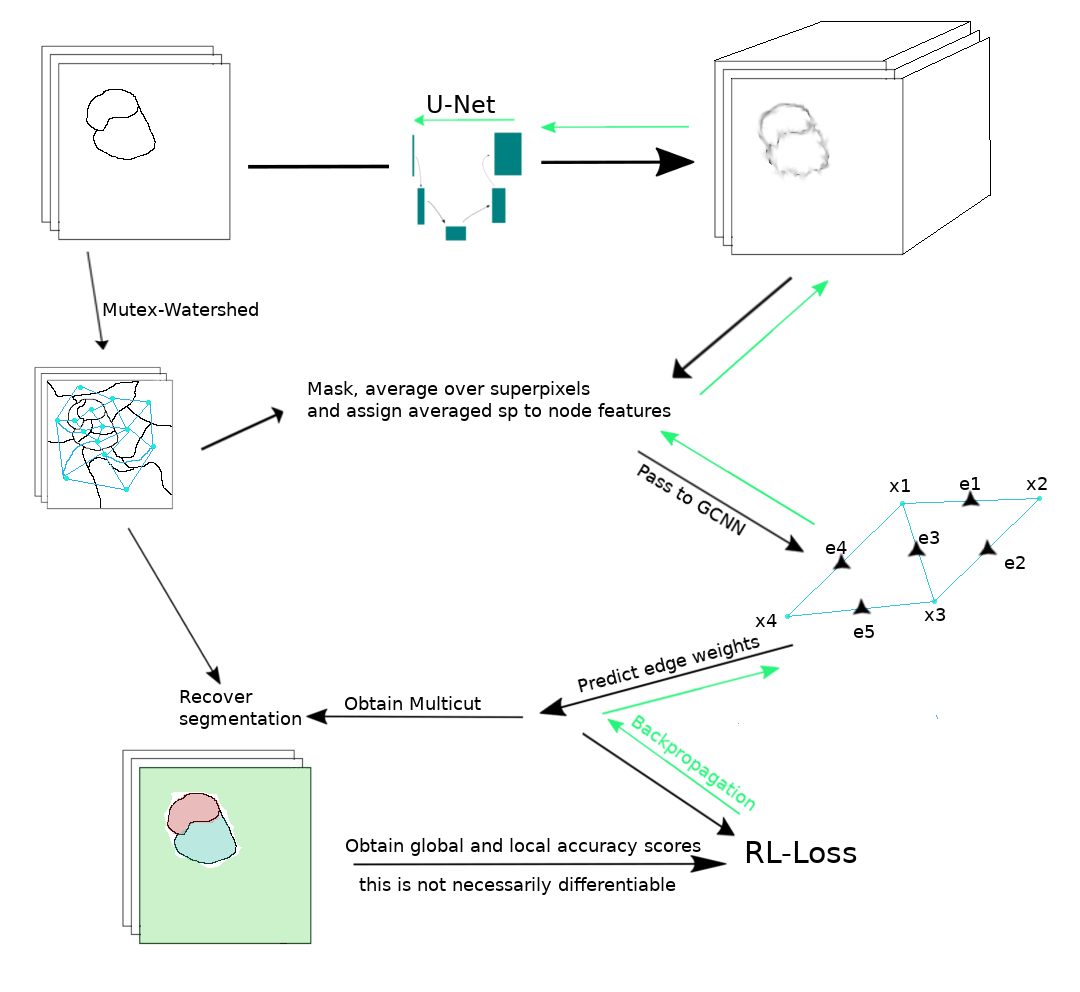
\includegraphics[width=1\textwidth]{figures/images/sketch_overall.png}
	\caption{Rough sketch of the proposed pipeline. Starting from raw data (top left), a superpixel graph is obtained with mutex watershed \ref{algo:mtx_wtsd} and pixel embeddings (top right) with an embedding network. Computing node features based on the average pixel embedding per superpixel a GCNN predicts logits on the edges of the superpixel graph. The logits are used to compute chances which in turn are used to compute costs based on which a multicut of the superpixel graph is computed and a segmentation is obtained from the multicut and the region adjacency graph of the superpixels. This segmentation is then evaluated and a reward is produced which is then used in the RL loss.}
	\label{overview}
\end{figure}


The following sections go into detail of every part in the sketch \ref{overview}